\documentclass[12pt,a4paper]{article}
\usepackage{amsmath}
\usepackage{amsfonts}
\usepackage{amssymb}
\usepackage{graphicx}
\usepackage[left=2cm,right=2cm,top=2cm,bottom=2cm]{geometry}

\author{Shyam Kumar P}
\title{Real Gas Equation}

\date{June 10, 2023}

\begin{document}

\maketitle

\section{ME22B223}
\textbf{Name}-Shyam Kumar P

\textbf{Roll No}-ME22B223

\textbf{Github User ID}-ShyamKumarP


\section{Introduction}
Under “model” gases, the systems are implied for
which state equations P = f(T, V) are derived under
particular assumptions concerning a molecule
dimensions and their interaction. Specifically, to such
gases refer the following “model” systems \footnote{This is referred from the contents present in \cite{sobko2014description}}: 

\begin{enumerate}
    \item The Van-der-Waals equation:
    \begin{equation}
        (V-b)(P+\frac{a}{V^2})=RT
    \end{equation}
    \item The Berthelot equation:
    \begin{equation}
        (V-b)(P+\frac{a}{V^2T})=RT
    \end{equation}
    \item The first Dieterici equation:
    \begin{equation}
        (V-b)P=RTe^{-\frac{a}{RTV}}
    \end{equation}
    \item The second Dieterici equation:
    \begin{equation}
        (V-b)(P+\frac{a}{V^\frac{5}{3}})=RT
    \end{equation}
\end{enumerate}

All the equations \footnote{This is referred from the contents present in  \cite{kondepudi2014modern}} are written for a one mole of
substance and reduced to a dimensionless form.In the present paper,
only the Van-der-Waals and their generalizations are considered.

\section{Understanding more about Real Gases}
Real Gas show deviation from the ideal gas law because molecules interact with each others.At high pressure molecules of gases are very close to each other resulting in molecular interactions.This causes a drag force on each other due to which molecules do not strike the wall of the container with full impact.

\begin{equation}
    P_{ideal} = P_{real} + \frac{an^2}{V^2}
    \label{precorrection}
\end{equation}

Here a is constant and second term of right hand side is a correction term for pressure.

Repulsive forces also become significant when molecules are almost in contact.The repulsive forces cause the molecules to behave as small but impenetrable spheres.The volume occupied by the molecules also becomes significant becomes instead of moving in volume V,these are now restricted to volume (V-nb) where nb is approximately the total volume occupied by the molecules themselves.

\begin{equation}
    V_{ideal} = V_{real} - nb
    \label{volcorrection}
\end{equation}

Here b is constant and second term of right hand side is a correction term for volume.

\begin{figure}
    \centering
    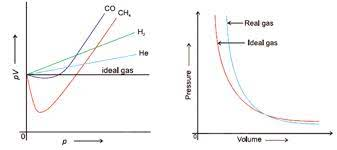
\includegraphics[width=\linewidth]{download.png}
    \caption{Caption}
    \label{fig:enter-label}
\end{figure}

\section{Deviation from ideal behaviour}
Real Gas show deviation from the ideal gas law because molecules interact with each other. At high pressure molecules of gases are very close to each other resulting in molecular interactions. This causes a drag force on each other due to which molecules do not strike the wall of the container with full impact. Also, at very low temperatures, intermolecular forces become significant. As the molecules travel with low average speed, these can be captured by one another due to attractive forces.

The deviation from ideal behavior can be measured in terms of compressibility factor Z, which is the ratio of product PV and nRT.Mathematically

\begin{equation}
    Z = \frac{PV}{nRT}
\end{equation}

For ideal gas $Z=1$ at all temperatures and pressures because PV=nRT. The graph of Z vs P will be a straight line parallel to the pressure axis. For gases that deviate from ideality, the value of Z deviates from unity. At very low pressures all gases shown have $Z=1$ and behave as an ideal gas. At high pressure, all the gases have $Z > 1$. These are more difficult to compress. At intermediate pressures, most gases have $Z<1$.

\begin{figure}[h]
    \centering
    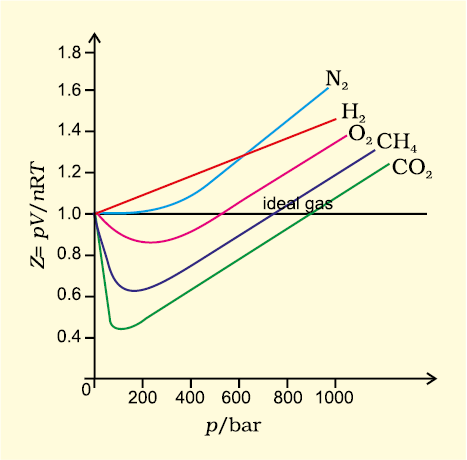
\includegraphics{Fig5_10.png}
    \caption{Variation of compressibility factor for some gases}
    \label{fig:enter-label}
\end{figure}

\section{Van der Waals Equation}

The van der Waals equation provides a more accurate description of real gases compared to the ideal gas law, especially at high pressures and low temperatures where intermolecular forces and molecular size effects become significant. The ideal gas equation after all the corrections like pressure correction (eqn~\ref{precorrection}) and volume correction (eqn~\ref{volcorrection}) becomes valid for real gas also. 

\begin{equation}
	\text(P + \frac{an^2}{V^2})(V - nb) = nRT
        \label{Realgaseqn}
\end{equation}

Besides the standard quantities of pressure P, volume V, absolute temperature T and a number of moles n, along with the ideal gas constant R, van der Waals equation contains two absolutely new parameters. Here a \& b are constants. The equation~\ref{Realgaseqn} is known as Van der Waals equation. In this equation \textit{n} is number of moles of the gas and constant \textit{a} \& \textit{b} are called van der Waals constants and their value depends on the characteristic of a gas.

\begin{align}
    \textbf{Nomenclature}
\end{align}
\begin{itemize}
\item a,b - constants
\item P - pressure
\item V - volume
\item T - temperature
\item R - universal gas constant (8.314 joules per kelvin per mole)
\end{itemize}

One is the covolume b,  the  molar  volume  occupied  by  the  molecules  or  atoms  in  the  gaseous  phase,  that  must  be  subtracted from the total volume of the container to obtain the free volume avail-able to the moving molecules. Van der Waals assumed such a volume to be equal to 4 times the actual molar volume of the molecules.Gases can be liquefied by reducing the pressure on them. When the pressure is reduced, the gas molecules have more space between them and can move more freely. This increased freedom of movement allows the gas molecules to move more quickly and to collide with each other more often. When the molecules collide with each other often, they begin to stick together, and the gas liquefies.

But the most interesting parameter is the second one, a. It specifies how much the pressure of the gas must be numerically increased in order to reproduce the ideal behavior. This means to assume that a sort of negative pressure acts between molecules,that opposes the translational, or motional, pressure exerted by the gas on the external walls. Therefore, molecules interact via attractive forces that however can reduce their capability for relative motion and diminish the pressure they can exert\footnote{This is refered from the contents present in \cite{della2022van}}. From an experimental point of view, the van der Waals parameters are related to the critical conditions, where van der Waals function P(V, T) at constant T has a point of inflection as a function of V, and defines the curve below which the gas phase comes in equilibrium with the liquid phase (Figure~\ref{fig:enter-label}).

Individual gas molecules do not have access to the total
volume \textit{v}, since the remaining molecules already occupy volume \textit{b}. The
correction term, $a/v^2$ at the pressure \textit{p}, implies that the kinetic energy with
which the molecules hit the volume boundary is lower than their kinetic
energy in the interior, owing to the attractive force of the molecules \footnote{This is referred from the contents present in \cite{langbein2006theory}}. The
attractive correction term in kinetic energy, velocity and pressure is
proportional to $1/v^2$, i.e. proportional to $1/r^6$ if \textit{r} is the mean separation
of the gas molecules.


\begin{figure}[h]
    \centering
    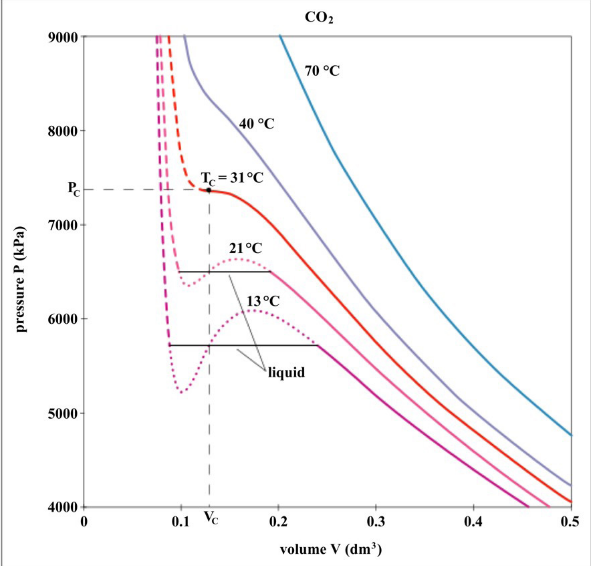
\includegraphics{Comparison.png}
    \caption{Comparison between the typical appearance of real gas isotherms (in the case of carbon dioxide) and that predicted according to van der Waals model.}
    \label{fig:enter-label}
\end{figure}

\bibliographystyle{plain}
\bibliography{myreferences}

\end{document}

